\documentclass[preprint]{elsarticle}
\usepackage[utf8]{inputenc}
\usepackage{amsmath}
\usepackage{amsfonts}
%\usepackage{tikz}
%\usetikzlibrary{shapes.misc,shadows}
%\usetikzlibrary{positioning} 
\usepackage{amsthm}
\usepackage{array}
\usepackage{parskip}
\usepackage{float}
\usepackage{paralist}
\usepackage{listings}
\usepackage{color}
\usepackage{caption}
\usepackage{hyperref}
\usepackage{multirow}
\usepackage{caption}
\usepackage{subcaption}
\usepackage{tikz}
\usetikzlibrary{shapes.misc,shadows}
\usetikzlibrary{quotes,positioning,arrows,decorations.markings}
\usetikzlibrary{positioning} 
\usepackage[cache=false,section]{minted}
\usepackage[a4paper, total={6in, 8in}]{geometry}
\usepackage[tworuled,algosection,figure,linesnumbered]{algorithm2e}
\usepackage{glossaries}
\usemintedstyle{default}
\newminted{haskell}{frame=lines,framerule=2pt}
\newminted{R}{frame=lines,framerule=2pt}
\graphicspath{{./images/}}

\bibliographystyle{abbrvnat}

\makeglossaries

\newacronym{dp}{DP}{Dynamic Pipeline Paradigm}
\newacronym{bfs}{BFS}{Breadth-First Search}
\newacronym{dfs}{DFS}{Depth-First Search}
\newacronym{wcc}{WCC}{Weak Connected Components}
\newacronym{hs}{Haskell}{Haskell Programming Language}
\newacronym{fp}{FP}{Functional Programming}
\newacronym{rl}{R}{R Language}
\newacronym{os}{OS}{Operative System}
\newacronym{dm}{Dm}{Diefficency Metrics}
\newacronym{tfft}{TFFT}{Time for the first tuple}
\newacronym{et}{ET}{Execution Time}
\newacronym{comp}{Comp}{Completeness}
\newacronym{tt}{T}{Throughput}
\newacronym{dt}{dief$@$t}{Diefficiency first $t$ time units}


\newtheorem{thm}{Theorem}
\newtheorem{lem}[thm]{Lemma}
\newdefinition{prob}{Problem}
\newdefinition{defin}{Definition}
\newdefinition{rmk}{Remark}
\newproof{pf}{Proof}
\newproof{pot}{Proof of Theorem \autoref{thm2}}

%\title{Towards a Haskell Abstraction of Dynamic Pipeline %Paradigm\tnoteref{t1}}

\title{Towards a Dynamic Pipeline Framework implemented in (parallel) Haskell\tnoteref{t1}}

\tnotetext[t1]{This work has been partially supported by funds from the Spanish Ministry for Science and Innovation and the European Union (FEDER funds) under grant MOTION (ref. TINXXXXXXXX)}
%
\author[1]{Juan Pablo Royo Sales}
\ead{juan.pablo.royo@estudiantat.upc.edu}

\author[1]{Edelmira Pasarella}
\ead{edelmira@cs.upc.edu}

\author[1]{Cristina Zoltan}
\ead{zoltan@cs.upc.edu}

\author[2]{Maria-Esther Vidal}
\ead{maria.vidal@tib.eu}

\affiliation[1]{organization={Universitat Politecnica de Catalunya},
postcode={08034},
city={Barcelona},
country={Spain}}

\affiliation[2]{organization={TIB/L3S Research Centre at the University of Hannover},
%addressline={JWRA 34, Jagathy},
%postcode={695014},
city={Hannover},
country={Germany}}

\begin{document}

\begin{abstract}
Data streaming processing has giving rise to new computation paradigms to provide effective and efficient processing of data streams. The most important features of these new paradigms is the exploitation of  the parallelism, the capacity of adapting execution schedulers, reconfigure computational structures, adjust the use of resources according to the characteristics of the input stream and produce incremental results. The Dynamic Pipeline Paradigm is a naturally functional approach to deal with stream processing. This fact encourages us to use a  pure functional programming language to implement a Dynamic Pipeline Framework (DPF).  In this work we tackled the problem of assessing the suitability of using (parallel) Haskell to implement a DPF.  The justification of this choice is twofold: From a formal point of view, Haskell has strong theoretical foundations providing the possibility of manipulating computations as primary entities and, from a practical point of view,  it has a powerful set of tools for writing multithreading and parallel computations with optimal performance. Firstly, we conduct an empirical evaluation to assess the performance of an \textit{ad-hoc} Haskell implementation of a naive dynamic pipeline to compute  the weak connected components of a graph (WCC).  After analyzing the results of the empirical evaluation we obtained insights on  the basis to construct parallel solutions using the Dynamic Pipeline Paradigm and the more relevant  factors that impact its scalability.  This allowed us to isolate which are the Haskell abstractions to be redefined and which new ones must be defined as well as the systems parameters to be considered to lift the WCC dynamic pipeline to a general  DPF implementation. Finally, we present a first approach of a general parametric DPF implementation.

%\textit{\acrfull{dp}} has been defined in order to solve problems where the data is heterogeneous 
%and in motion. Taking advantage on pipelining stage parallelization, this paradigm allows to dynamically adapt 
%stage computations according to the input. It has been shown in the definition of this computational model that any
%implementation attempt of the paradigm requires fast and flexible parallelization techniques as well as tools that 
%are suitable with the notion of computation as a \emph{first-class citizen}. In this work, we implement the \textit{Dynamic Pipeline Paradigm}
%in \texttt{Haskell} for solving the problem of finding \textit{Connected Components of a Graph}. We experiment with different kind of Graphs and show how %\texttt{Haskell} behaves on that context. Through this approximation we generate enough evidence to support that \texttt{Haskell} it is a suitable Language %for implementing \textit{Dynamic Pipeline Paradigm} not only because of its strong theoretical foundations which provides different Abstraction to manipulate %computations as primary entities with Mathematical reasoning, but also because it has a powerful Set of Tools for writing multithreading and parallel %computations.
\end{abstract}

\begin{keyword}
Dynamic pipeline \sep Haskell \sep parallelism \sep concurrency
\end{keyword}

\maketitle

\section{Introduction}
Traditionally, \acrfull{hs} has been considered as an academic language instead of a production language. However it is lastly well known that in addition to its strong theoretical foundations it has a powerful set of tools for writing multithreading and parallel programs with optimal performance.

On the other hand, \textit{\acrfull{dp}} \cite{dpdef} offers a promising model for Big Data Streaming Processing taking advantage of Pipeline Parallelization. 

One of the biggest challenge of \acrshort{dp} is to find a proper set of tools and programming language which can take advantage from both: \begin{inparaenum}[i\upshape)]
\item  \emph{fast parallel} processing and 
\item  \emph{strong theoretical} foundations that manage computations as first-class citizens.
 \end{inparaenum}

On this work, we conduct an implementation of \acrshort{dp} for solving \acrfull{wcc} with \acrshort{hs} showing that both aspects mentioned can be covered with \acrshort{hs}. At the same time we run some experiments to validate our assumptions about the feasibility of the chosen language, as well as providing a first approximation Design of a General Purpose \acrshort{dp} Library in \acrshort{hs}.

\textbf{Problem Research and Objective:}\label{research:obj} The main objective of this work is to explore the feasibility of using a  \acrfull{fp} language to implement the \acrfull{dp} model of computation. In particular, we tackle the problem of establishing the basis of a implementation of the \emph{Dynamic Pipeline} computation model in \acrfull{hs}, a pure functional language. This is,  we want to determine the particular features (including versions, libreries, etc) of this language that will allow us to go beyond a simple experimental implementation of a \acrshort{dp}. To be concrete, by means of a particular and very relevant problem as the computation of the \acrfull{wcc} of a graph,  we study the two critical features required and mentioned above in a \acrshort{dp} \acrshort{hs} for a \acrshort{dp} model implementation.

\textbf{Approach:} In the first section of our work we present the \emph{Motivation Example} that is conducting this work (\acrshort{wcc}). Following that we define \acrshort{dp} Paradigm and at the same time we expose what are the premises that support \acrshort{hs} as a suitable language for this implementation.
In the next part we are going to show the details of the Implementation that we have done in \acrshort{hs} to solve the \emph{Motivating Example} proposed. In addition to that we present our \emph{Empirical Evaluation} which are going to answer our Hypothesis.
Finally we show the \emph{First Approximation} of the Design of a \emph{Dynamic Pipeline Framework} implemented in \acrshort{hs}.

\textbf{Contributions:} Show \acrshort{hs} is a suitable Language for implementing \acrshort{dp}, generating enough evidence through an Empirical Evaluation based on a Example problem (\acrshort{wcc}). This work also contribute in building the first abstraction approximation of \acrshort{dp} in \acrshort{hs} as a future Framework/Library of this Computational Model in that Language. 


\section{Preliminaries}\label{section:prelim}
\subsection{Dynamic Pipeline Paradigm}\label{sub:sec:dp:par}
%
Stream Programming has became very popular and there are several frameworks that support it  based on the model of pipelines, fork, and join operators Spark \cite{apachespark}, Knime \cite{knime}, Hadoop \cite{hadoop}, etc. Algorithmic solutions based on this frameworks consists in describing dependencies among pieces of sequential  code/actors. To our knowledge, very few frameworks have constructions that allow programmers to express a pipeline having a variable length during program execution. A \textit{Dynamic Pipeline  (DP)}  \cite{dpdef} is a data-driven one-dimensional and unidirectional chain of stages connected by means of channels synchronized by data availability. This computational structure stretches and shrinks depending on the spawning and the lifetime of its stages, respectively. Modeling an algorithmic solution as a DP corresponds to define a dynamic computational structure  in terms of four kind of stages:  \textit{Input},  \textit{Generator},  \textit{Output} and \textit{Filter} stages.  To be concrete, the parameterized actors (algorithms)  corresponding to the behavior of each of these stages must be defined as well as the number and the type of the I/O channels connecting them. Channels are unidirectional  according to the flow of the data. Before executing an algorithm deployed as a  DP, the initial configuration of the pipe must be stated. This is, an initial pipe composed of a chain of instantiated stages: \textit{Input},  \textit{Generator} and \textit{Output}. \autoref{fig:initialpipe_wcc} depicts the initial state of a DP.  As data are incoming  the \textit{Generator} stage spawns \textit{Filter} stage instances. \textit{Filters} contains the actor(s) that occur when solving a problem. \autoref{fig:active_wcc_2nd_inp} illustrates this case.
%
\subsection{Motivating Example}\label{sub:sec:mot:ex}
We have selected \acrfull{wcc} as a motivational example problem for conducting this work. This has been already described in previous \acrshort{dp} work \citep{dpdef} as one of the suitable problems to be solve by this Paradigm.

\begin{defin}
A connected component of a graph $G$ is a connected subgraph $S$ of $G$ that is not a proper subgraph
of another connected subgraph $S'$ of $G$. Therefore, a connected component of a graph $G$ is a maximal
connected subgraph of $G$.
\end{defin}

Given an undirected graph $G = (V, E)$, we can find \acrshort{wcc} of $G$ in $O(V + E)$ using \textit{\acrfull{dfs}} or \textit{\acrfull{bfs}} algorithm \citep{CormenLeisersonEtAl09}. 

Although this problem can be solved in linear time, when we are manipulating real-world graphs, which are usually big, it would be better to have a computational model where this can be processed faster. \acrshort{dp} with its \textit{Parallelization Pipeline model} improve that speed up on Big Graphs for finding \acrshort{wcc}.

Although this example does not present many challenges at algorithmic level, we consider a proper problem to explore our assumptions because of the following:

\begin{itemize}
    \item It allows us to compare \acrshort{dp} implementation against default implementation with \acrshort{dfs} and explore the difference in execution time between both
    \item It allows us to describe a simple algorithm on \acrshort{dp} model without expending efforts of solving some complex algorithmic problem which is not the main objective of this work
    \item It allows us to validate the correcteness of the implementation with \acrshort{dp} because of the first statement.
\end{itemize}


%
\tikzset{source/.style={shape=rectangle, minimum size=8mm}}
\tikzset{ionode/.style={shape=rectangle, draw=blue!50, fill=blue!5, very thick, minimum size=8mm, drop shadow={opacity=.5,shadow xshift=0pt}}}
\tikzset{ionode/.style={shape= rectangle, draw=blue!50, fill=blue!5, very thick, minimum size=8mm,drop shadow={opacity=.5,shadow xshift=0pt}}}
\tikzset{gennode/.style={shape= rectangle, draw=gray!50, fill=gray!5, very thick, minimum size=8mm, drop shadow={opacity=.5,shadow xshift=0pt}}}
\tikzset{filternode/.style={shape=rectangle, draw=cyan!50, fill=white, very thick, minimum size=8mm,drop shadow={opacity=.5,shadow xshift=0pt}}}
\tikzset{paramnode/.style={shape=rectangle, draw=cyan!50, fill=white, very thick, minimum size=8mm, 
drop shadow={opacity=.5,shadow xshift=0pt}}}
\tikzset{edge/.style = {->,> = latex}}
\tikzstyle{ioedge} = [thick, decoration={markings,mark=at position
   1 with {\arrow[semithick]{open triangle 60}}},
   double distance=1.4pt, shorten >= 5.5pt,
   preaction = {decorate},
   postaction = {draw,line width=1.4pt, white,shorten >= 4.5pt}]

%
%%%%%%%%% Subfigures %%%%%%
%
\begin{figure}[!hb]
    \centering
     \begin{subfigure}[b]{0.5\textwidth}
     	\centering
	\begin{tikzpicture}
	%Nodes
	\node[source]      (stream)                  {\mbox{{\small $eof\: (3,4) \: (4,5) \: (3,6)$}}};
	\node[ionode]      (in)                    [right=of stream]      {\textit{\bf I}};
	\node[gennode]   (gen)                [right=of in] {\textit{\bf G}};
	\node[ionode]      (out)                 [right=of gen] {\textit{\bf O}};
	\node[filternode]  (filter)                [above= 0.2mm of gen] {\textit{\bf F}};
	%Lines
	\draw[ioedge] (stream) to (in);
	\draw[edge] (in.15) to ["{\small $(1,2)$ }"] (gen.166);
	\draw[edge] (in.-15) to (gen.195);
	\draw[edge] (gen) to (out);
	\end{tikzpicture}
	\caption{{\bf Initial configuration of a Dynamic Pipeline.} First element source} 
	\label{fig:initialpipe_wcc}
	\end{subfigure}
    	\hfill
%
     \begin{subfigure}[b]{0.5\textwidth}
         \centering
	\begin{tikzpicture}
	%Nodes
	\node[source]      (stream)                  {{\small $eof\: (3,4) \: (4,5)$}};
	\node[ionode]      (in)                     [right=of stream]        {\textit{\bf I}};
	\node[filternode]  (filter1)               [right=of in] {\small $\{1,2\}$};
	\node[gennode]   (gen)                 [right=of filter1] {\textit{\bf G}};
	\node[paramnode]  (param)          [above= 0.2mm of gen] {\textit{\bf F}};
	\node[ionode]      (out)                  [right=of gen] {\textit{\bf O}};
	%Lines
	\draw[ioedge] (stream) to (in);
	\draw[edge] (in.15) to ["{\small$(3,6)$}"] (filter1.168);
	\draw[edge] (in.-15) to (filter1.191);
	\draw[edge] (filter1.11) to (gen.166);
	\draw[edge] (filter1.-13) to (gen.196);
	\draw[edge] (gen) to (out);
	\end{tikzpicture}
	\caption{{\bf Dynamic Pipeline with some filter instances.} Second element source} 
	\label{fig:active_wcc_2nd_inp}
	\end{subfigure}
	\hfill
%
\begin{subfigure}[b]{1.0\textwidth}
	\centering
	\begin{tikzpicture}
	%Nodes
	\node[source]      (stream)                  {{\small $eof\: (3,4)$}};
	\node[ionode]      (in)                     [right=of stream]        {\textit{\bf I}};
	\node[filternode]  (filter1)               [right=of in] {\small $\{1,2\}$};
	\node[gennode]   (gen)                 [right=of filter1] {\textit{\bf G}};
	\node[paramnode]  (param)          [above= 0.2mm of gen] {\textit{\bf F}};
	\node[ionode]      (out)                  [right=of gen] {\textit{\bf O}};
	%Lines
	\draw[ioedge] (stream) to (in);
	\draw[edge] (in.15) to ["{\small$(4,5)$}"] (filter1.168);
	\draw[edge] (in.-15) to (filter1.191);
	\draw[edge] (filter1.11) to ["{\small$(3,6)$}"] (gen.166);
	\draw[edge] (filter1.-13) to (gen.196);
	\draw[edge] (gen) to (out);
	\end{tikzpicture}
	\caption{{\bf Dynamic Pipeline with some filter instances.} Third element source} 
	\label{fig:active_wcc_3rd_inp}
	\end{subfigure}
	\hfill
%
	\begin{subfigure}[b]{1.0\textwidth}
	\centering
	\begin{tikzpicture}
	%Nodes
	\node[source]      (stream)                  {{\small $eof$}};
	\node[ionode]      (in)                     [right= of stream]        {\textit{\bf I}};
	\node[filternode]  (filter1)               [right=of in] {\small $\{1,2\}$};
	\node[filternode]  (filter2)               [right=of filter1] {\small $\{3,6\}$};
	\node[gennode]   (gen)                 [right=of filter2] {\textit{\bf G}};
	\node[paramnode]  (param)          [above= 0.2mm of gen] {\textit{\bf F}};
	\node[ionode]      (out)                  [right=of gen] {\textit{\bf O}};
	%Lines
	\draw[ioedge] (stream) to (in);
	\draw[edge] (in.15) to ["{\small$(3,4)$}"] (filter1.168);
	\draw[edge] (in.-15) to (filter1.191);
	\draw[edge] (filter1.11) to ["{\small$(4,5)$}"] (filter2.170);
	\draw[edge] (filter1.-13) to (filter2.194);
	\draw[edge] (filter2.11) to  (gen.167);
	\draw[edge] (filter2.-13) to (gen.196);
	\draw[edge] (gen) to (out);
	\end{tikzpicture}
	\caption{{\bf Dynamic Pipeline with some filter instances.} Fourth element source} 
	\label{fig:active_wcc_4th_inp}
	\end{subfigure}
	\hfill
%
    \caption{WCC-Dynamic Pipeline Example. First round}
    \label{fig:wcc-dp-1}
\end{figure}
%
%
%
\begin{figure}[!hb]
    \centering
%
	\begin{subfigure}[b]{1.0\textwidth}
	\centering
	\begin{tikzpicture}
	%Nodes
	\node[source]      (stream)                  {\hspace{1cm}};
	\node[filternode]  (filter1)               [right=of stream] {\small $\{1,2\}$};
	\node[filternode]  (filter2)               [right=of filter1] {\small $\{3,6\}$};
	\node[gennode]   (gen)                 [right=of filter2] {\textit{\bf G}};
	\node[paramnode]  (param)          [above= 0.2mm of gen] {\textit{\bf F}};
	\node[ionode]      (out)                  [right=of gen] {\textit{\bf O}};
	%Lines
	\draw[edge] (stream.16) to ["{\small$eof$}"] (filter1.167);
	\draw[edge] (stream.-16) to ["{\small$eof$}",swap] (filter1.191);
	\draw[edge] (filter1.11) to ["{\small$(3,4)$}"] (filter2.170);
	\draw[edge] (filter1.-13) to (filter2.194);
	\draw[edge] (filter2.11) to ["{\small$(4,5)$}"] (gen.167);
	\draw[edge] (filter2.-13) to (gen.196);
	\draw[edge] (gen) to (out);
	\end{tikzpicture}
	\caption{{\bf Dynamic Pipeline with some filter instances.} Fifth element source} 
	\label{fig:active_wcc_5th_inp}
	\end{subfigure}
	\hfill
%
	\begin{subfigure}[b]{1.0\textwidth}
	\centering
	\begin{tikzpicture}
	%Nodes
	\node[source]      (in)                   {\hspace{1cm}};
	\node[source]      (stream)                 [right=of in]    {\hspace{1cm}};
	\node[filternode]  (filter2)               [right=of stream] {\small $\{3,4,6\}$};
	\node[filternode]  (filter3)               [right=of filter2] {\small $\{4,5\}$};
	\node[gennode]   (gen)                 [right=of filter3] {\textit{\bf G}};
	\node[paramnode]  (param)          [above= 0.2mm of gen] {\textit{\bf F}};
	\node[ionode]      (out)                  [right=of gen] {\textit{\bf O}};
	%Lines
	\draw[edge] (stream.17) to ["{\small$eof$}"] (filter2.170);
	\draw[edge] (in.-20) to  ["{\small$eof\:\{1,2\}$}",swap]   (filter2.190);
	\draw[edge] (filter2.10) to ["{\small$eof$}"] (filter3.169);
	\draw[edge] (filter2.-10) to  (filter3.194);
	\draw[edge] (filter3.12) to  (gen.167);
	\draw[edge] (filter3.-12) to (gen.196);
	\draw[edge] (gen) to (out);
	\end{tikzpicture}
	\caption{{\bf Dynamic Pipeline with some filter instances.} EOF2-1 source} 
	\label{fig:active_wcc_eof1_inp}
	\end{subfigure}
	\hfill
%
\begin{subfigure}[b]{1.0\textwidth}
	\centering
	\begin{tikzpicture}
	%Nodes
	\node[source]      (in)                   {\hspace{1cm}};
	\node[source]      (stream)                 [right=of in]    {\hspace{1cm}};
	\node[filternode]  (filter3)               [right=of stream] {\small $\{4,5\}$};
	\node[gennode]   (gen)                 [right=of filter3] {\textit{\bf G}};
	\node[paramnode]  (param)          [above= 0.2mm of gen] {\textit{\bf F}};
	\node[ionode]      (out)                  [right=of gen] {\textit{\bf O}};
	%Lines
	\draw[edge] (stream.17) to ["{\small$eof$}"] (filter3.168);
	\draw[edge] (in.-20) to  ["{\small$eof\:$\{3,4,6\}$\:\{1,2\}$}",swap]   (filter3.195);
	\draw[edge] (filter3.12) to  (gen.167);
	\draw[edge] (filter3.-12) to (gen.196);
	\draw[edge] (gen) to (out);
	\end{tikzpicture}
	\caption{{\bf Dynamic Pipeline with some filter instances.} EOF2-2 source} 
	\label{fig:active_wcc_eof2_inp}
	\end{subfigure}
	\hfill
%
\begin{subfigure}[b]{1.0\textwidth}
	\centering
	\begin{tikzpicture}
	%Nodes
	\node[source]      (in)                   {\hspace{1cm}};
	\node[source]      (stream)                 [right=of in]    {\hspace{1cm}};
	\node[filternode]  (filter3)               [right=of stream] {\small $\{4,5\}$};
	\node[gennode]   (gen)                 [right=of filter3] {\textit{\bf G}};
	\node[paramnode]  (param)          [above= 0.2mm of gen] {\textit{\bf F}};
	\node[ionode]      (out)                  [right=of gen] {\textit{\bf O}};
	%Lines 
	\draw[edge] (in.-20) to  ["{\small$eof\:\{3,4,6\}$}",swap]   (filter3.195);
	\draw[edge] (filter3.12) to  ["{\small$eof$}"] (gen.167);
	\draw[edge] (filter3.-12) to ["{\small$\{1,2\}$}",swap] (gen.196);
	\draw[edge] (gen) to (out);
	\end{tikzpicture}
	\caption{{\bf Dynamic Pipeline with some filter instances.} EOF2-3 source} 
	\label{fig:active_wcc_eof3_inp}
	\end{subfigure}
	\hfill
%
\begin{subfigure}[b]{1.0\textwidth}
	\centering
	\begin{tikzpicture}
	%Nodes
	\node[source]      (stream)                 {\hspace{1cm}};
	\node[filternode]  (filter3)               [right=of stream] {\small $\{3,4,5,6\}$};
	\node[ionode]   (gen)                 [right=of filter3] {\textit{\bf O}};
	\node[source]      (out)                 [right=of gen]    {\small $\{1,2\}$};
	%Lines
	\draw[edge] (stream.-20) to  ["{\small$eof$}",swap]   (filter3.190);
	\draw[edge] (filter3.-10) to  (gen.199);
	\draw[ioedge] (gen) to (out);
	\end{tikzpicture}
	\caption{{\bf Dynamic Pipeline with some filter instances.} EOF2-4 source} 
	\label{fig:active_wcc_eof4_inp}
	\end{subfigure}
	\hfill
%
\begin{subfigure}[b]{1.0\textwidth}
	\centering
	\begin{tikzpicture}
	%Nodes
	\node[source]      (in)                   {\hspace{1cm}};
	\node[source]      (stream)                 [right=of in]    {\hspace{1cm}};
	\node[ionode]   (gen)                 [right=of stream] {\textit{\bf O}};
	\node[source]      (out)                 [right=of gen]    {\small $\{1,2\}$};
	%Lines
	\draw[edge] (in.-21) to  ["{\small$eof\:\{3,4,5,6\}$}",swap]   (gen.199);
	\draw[ioedge] (gen) to (out);
	\end{tikzpicture}	
	\caption{{\bf Dynamic Pipeline with some filter instances.} EOF2-5 source} 
	\label{fig:active_wcc_eof5_inp}
	\end{subfigure}
	\hfill
%
\begin{subfigure}[b]{1.0\textwidth}
	\centering
	\begin{tikzpicture}
	%Nodes
	\node[source]      (stream)                  {\hspace{1cm}};
	\node[ionode]   (gen)                 [right=of stream] {\textit{\bf O}};
	\node[source]      (out1)                 [right=of gen]    {\small $\{3,4,5,6\}\:\{1,2\}$};
	\node[source]      (out2)                 [right=of out1]    {\small $\{3,4,5,6\}\:\{1,2\}$};
	%Lines
	\draw[edge] (stream.-21) to  ["{\small$eof$}",swap]   (gen.199);
	\draw[ioedge] (gen) to (out1);
	\end{tikzpicture}
	\caption{{\bf Dynamic Pipeline with some filter instances.} EOF2-6 source} 
	\label{fig:active_wcc_eof6_inp}
	\end{subfigure}
	\hfill
%

    \caption{WCC-Dynamic Pipeline Example. Second round}
    \label{fig:wcc-dp-2}
\end{figure}


\subsection{Haskell generalities}
\acrshort{hs} is a \emph{Statically Typed Pure Functional Language} which more than $30$ years of Academic Research implemented within the language, and widely used in different kind of solutions in the Industry as well such as \emph{Blockchain, Banks, Financial Institutions, APIs, tools, etc}. Some of the most important features in the language are: \textbf{Statically Typed, Pure Functional, Type inference, Lazyness and Concurrency.} \cite{haskell}

\acrshort{hs} implements \emph{System F} \cite{systemf} which is also known as \textit{polymorphic $\lambda$-calculus or the second-order $\lambda$-calculus} giving the language a strong theoretical roots. On the other hand all the past Academic Research years have been positively impacted in the evolution of the language giving birth to a lot of abstractions and other theoretical constructions that have been added as well, since the concept of \texttt{Monads} \cite{monads} and other \texttt{Category Theory} \cite{arrows} constructions up to \texttt{Dependent Types} \cite{dependenttypes} and \texttt{Effectfull Systems} \cite{extensibleeff} lately. 

\section{The Dynamic Pipeline Framework: First Approach}\label{section:prob:dp:haskell}
Implementing a model of computation such as \acrshort{dp} requires certain characteristics that host Language and tools should provide in order to reach the desired objective. In regards to this, and according to what has been described on \autoref{section:prelim} we can argue that some of those primary aspects should be:

\begin{itemize}
    \item \textbf{Filters}: Since our Model is meant to generate dynamic computations (functions), throughout the Pipeline processing life cycle, our Language should be be able to have \textit{Functions} as a \textit{first-class citizens}
    \item \textbf{Dynamic Stages}: According to the previous item, it is not only require a strong representation of computation or functions but as well some Abstractions that can represent this dynamic behaviour which enlarge and shrink the pipeline but in terms of functions and not only data.
    \item \textbf{Parallelization}: Another key aspect on this model 
    \item \textbf{Channels}: Communication between Dynamic Stages, represented as \textit{Channels} by the Model, is the last key component.
\end{itemize}

Using a Language like \acrshort{hs} fulfills completely all those requirements exposed before because of the following:

\begin{itemize}
    \item \textbf{Filters}: \acrfull{fp} Language like \acrshort{hs} it is a perfect host for representing those \textit{Dynamic Computations}, not only due to its \acrshort{fp} nature, but also for it is Strong Type System which ensure safeness on the data representation pipeline and the computational sequence.
    \item \textbf{Dynamic Stages}\label{dyn:stage}: Abstractions like \textbf{Recursive Schemes} \citep{lenses} has been deeply explored and used in \acrshort{hs} and allow us to represent in a formal and simple way \textit{dynamic} structure through \textit{Anamorphisms} and \textit{Catamorphisms}.
    \item \textbf{Parallelization}: Parallelization tehcniques and tools have also been intensively studied and implemented¡ in \acrshort{hs} \citep{monadpar} and it is well known that \acrshort{hs} light threads and spark allows to spawn thousands to millions of parallel computations without penalizing performance compare with \acrfull{os} level threading \citep{parallelbook}.
    \item \textbf{Channels}: As the last topic we have several techniques to our disposal to communicate between \textit{threads/sparks} in \acrshort{hs} like \mintinline{haskell}{MVar} or concurrent safe like \mintinline{haskell}{STM}. Moreover we have at our disposal \textit{Channels} abstractions based on both mentioned communication mechanisms. 
\end{itemize}

Having exposing that, those are the reason that we believe \acrshort{hs} suits well for implementing \acrshort{dp} Paradigm\footnote{All the Source Code of this work can be found here https://github.com/jproyo/upc-miri-tfm/tree/feature/library-v1/connected-comp}.

\subsection{Libraries and Tools}\label{sub:lib:tools}
In this part we show how is the abstraction approximation that we design to represent \acrshort{dp} model in \acrshort{hs}, but before showing the details it would be beneficial in order to understand the solution, to describe which libraries and tools have been decided to use.

As we have discussed before on \autoref{section:prob:dp:haskell}, there are at least 4 \emph{important aspects} in \acrshort{dp} design implementation to be covered: \begin{inparaenum}[i\upshape)]
\item \emph{Filters}
\item \emph{Dynamic Stages}
\item \emph{Parallelization}
\item and \emph{Channels}
 \end{inparaenum}.

\textbf{\textit{Filters}}\label{sub:sec:filter}: As we have discuss previously this is provided for free by the already built in language abstraction and the \acrshort{fp} paradigm itself where Functions are primary computational entities. Therefore there is no need to select any other additional library rather than using \emph{Monads} \citep{monads} for reflecting the Chain of Computations and the dependency between those computations, since we are implementing a Pipeline. In that sense if we represent \acrshort{dp} model as a \emph{Monad} we are getting for free the guarantee of \emph{Monad Laws}, in in particular \emph{Associativity law} which state that $(m >>= f ) >>= g = m >>= (\lambda x.f x >>= g)$ \citep{monadlaws}.

\textbf{\textit{Dynamic Stages}}: As well as in the previous point on \autoref{sub:sec:filter}, this is another abstraction that is already provided in the base library through the use of \mintinline{haskell}{fold} and \mintinline{haskell}{unfold} combinators which are the equivalent of \emph{Catamorphism} and \emph{Anamorphism} respectively. In this first approximation, we have chosen the simplest abstraction but as we mentioned before on \autoref{dyn:stage}, we believe that if we implement in a future work a proper \emph{Recursive Scheme} we can benefit of other properties and laws that those \emph{Fix Point Algebra and CoAlgebra Structures} \citep{lenses} provides. 

\textbf{\textit{Parallelization}}: One of the most important components on the implementation is the selection of \emph{Concurrency Library} to support an intensive parallelization workload. A direct guess to achieve this could be to use \textit{monad-par} library based on this work \citep{monadpar}, but we have discarded it because the Parallelism it is needed to be achieved is at \emph{Thread level} and not at \emph{Spark level} \cite{sparks}, due to the nature of \acrshort{dp}, where Pipeline Parallelism and not Data Parallelism is structural processing mechanism. The next obvious choice is to use \mintinline{haskell}{forkIO :: IO () -> IO ThreadId} from \mintinline{bash}{base} library \cite{forkio}, but that would imply to handle all the threads lifecycle, terminations and errors programmatically without major combinators or abstractions to deal with it. Therefore, we choose \textbf{async} \cite{async}
library which allow us to spawn asynchronous computations \citep{parallelbook} on \acrshort{hs} and at the same time provides usefull combinators to managing thread terminations and errors.

\textbf{\textit{Channels}}\label{section:channels}: Finally the use of \emph{Channels} as a communication mechanism between Dynamic Stages and Data flowing in \acrshort{dp} model are implemented using \textbf{unagi-chan} \cite{unagi} library which provides the following advantages to our solution:

\begin{itemize}
  \item \mintinline{haskell}{MVar} Channel with \textbf{no} use of \mintinline{haskell}{STM}: This allows to avoid internal locking for concurrent access. In this case
  we can use this advantage because in \acrshort{dp} model, one specific \textit{Pipeline Stage} which is running in a separated thread can only access to its \textit{Inputs/Outputs} channels for \textit{Reading/Writing} accordingly 
  and those operations are not concurrently share by other Threads (\textit{Stages}) for the same Channels.  
  \item \textbf{Non-Blocking} Channels: This library contains blocking and non-blocking Channels for reading and this is a key aspect to gain performance and speed up on the implementation.
  \item Optimized for $x86$ Architectures with use of low-level \textit{fetch-and-add} instructions.
  \item $100x$ faster on Benchmarking compare with \mintinline{haskell}{STM} and default base \mintinline{haskell}{Chan} implementations.
\end{itemize}

\section{A Connected Component Dynamic Pipeline Implementation}

\subsection{DP Haskell Principal Algorithm}

The following is the principal algorithm which represents the \textit{Monadic} computational chain of \acrshort{dp} main three \textit{Stages}: \begin{inparaenum}[i\upshape)]
\item \emph{Input}
\item \emph{Generator}
\item \emph{Output}
 \end{inparaenum}.

\begin{listing}[H]
\begin{minted}[fontsize=\small,numbers=left,frame=lines,framerule=2pt,framesep=2mm,baselinestretch=1.2,highlightlines={2,11}]{haskell}

runParallelDP :: Handle -> IO ()
runParallelDP h = input h >>= generator >>= output

input :: Handle -> IO (DP.Stream Edge ConnectedComponents)
input h = fromInput h >>= (|>> parseEdges)

output :: ConnCompDP -> IO ()
output = DP.mapM (R.putStrLn . show)

fromInput :: Handle -> IO (DP.Stream ByteString ConnectedComponents)
fromInput h = DP.unfoldM (B.hGetLine h) (R.hIsEOF h)

parseEdges :: ByteString -> IO [Edge]
parseEdges = toEdge . decodeUtf8

\end{minted}
\caption{Main algorithm \acrshort{dp} for \acrshort{wcc}}
\label{src:haskell:1}
\end{listing}

It can be seen in the \textbf{line 3} that the implementation of \acrshort{dp} in \acrshort{hs} matches almost identically to the formal definition of proposed paradigm model.

We can also appreciate in the \textbf{line 12} the use of the \mintinline{haskell}{unfoldM} which is the \emph{Anamorphism} that is reading incrementally from the \emph{Input File} and creating the Stream.

It is important to notice that the input is being read in \textbf{non-blocking} mode and by batches of bytes\footnote{In this particular case by line because of parsing conveniences} allowing the streaming computation processing the edges as long as it arrives to the \textit{Generator} or the first \textit{Filter} Stages.\footnote{The format of the input file for the case of this example is an \textbf{edgelist} format compatible with \emph{igraph R library} or similar https://igraph.org/r/doc/write\_graph.html}

\subsection{DP Connected Components in Haskell}
In this subsection we are going to describe how we have implemented \acrshort{wcc} algorithm in \acrshort{dp} model with \acrshort{hs}. Once we have the main components and the abstraction setup we only need to define how the \mintinline{haskell}{generator} function needs to behave and what the \textbf{filters} internally needs to do to process arriving data. 

\textbf{Generator:}\newline
The \textit{Generator} is the Computation in the Pipeline which is responsible to know when to interpose a new \textit{Filter} in front of the Pipe on \autoref{sub:sec:dp:par}.
In the case of \acrshort{wcc} a new \textit{Filter} is created on each new Edge that arrives to the \textit{Generator}.

\begin{listing}[H]
\begin{minted}[fontsize=\small,numbers=left,frame=lines,framerule=2pt,framesep=2mm,baselinestretch=1.2,highlightlines={2,11}]{haskell}
generator :: ConnCompDP -> IO ConnCompDP
generator = DP.foldrS createNewFilter
  where
    createNewFilter c v = do
      newInput  <- newChan
      newOutput <- newChan
      DP.Stream newInput newOutput 
            <$> async (newFilter (toConnectedComp v) c newInput newOutput)
  
  \end{minted}
  \caption{Generator \acrshort{dp} for \acrshort{wcc}}
  \label{src:haskell:2}
\end{listing}

As we can appreciate here, the highlighted \textbf{line 2} shows the use of the \acrshort{hs} \textit{Catamorphism} which it is reducing the \textit{Stream} and at the same time creating the intermediate \textit{Filters} (Stages) of the Pipe.

\textbf{Filters:}\newline
In this case the algorithm is not as succinct as the previous because here is where the 2-step calculation takes place. As we have explained before each \textit{Filter} contains 2 sequential computations which are called \mintinline{haskell}{actor1} and \mintinline{haskell}{actor2}. The first one is responsible for gathering Connected Components based on the first Edge this \textit{Filter} was created from, and the second \textit{Actor} is responsible for \textit{combining} its own calculated Connected Components with others that are coming from the downstream. Representing sequential computations in \acrshort{hs} is simple with \emph{Monadic} computations, which in this case \mintinline{haskell}{actor2} depends on the computation of \mintinline{haskell}{actor1}.

\begin{listing}[H]
\begin{minted}[fontsize=\small,numbers=left,frame=lines,framerule=2pt,framesep=2mm,baselinestretch=1.2,highlightlines={3,10-11,21-22}]{haskell}
newFilter :: ConnectedComponents -> ConnCompDP 
          -> DP.Channel Edge -> DP.Channel ConnectedComponents -> IO ()
newFilter conn inCh toInCh outCh = actor1 conn inCh toInCh >>= actor2 inCh toInCh outCh

actor1 :: ConnectedComponents -> ConnCompDP -> DP.Channel Edge -> IO ConnectedComponents
actor1 conn inCh toInCh = maybe finishActor doActor =<< DP.pullIn inCh
 where
  finishActor = DP.end' toInCh >> return conn

  doActor v | toConnectedComp v `intersect` conn = actor1 (toConnectedComp v <> conn) inCh toInCh
            | otherwise                          = v `DP.push'` toInCh >> actor1 conn inCh toInCh


actor2 :: ConnCompDP -> DP.Channel Edge 
       -> DP.Channel ConnectedComponents -> ConnectedComponents -> IO ()
actor2 inCh toInCh outCh conn = maybe finishActor doActor =<< DP.pullOut inCh

 where
  finishActor = conn `DP.push'` outCh >> DP.end' outCh

  doActor cc | conn `intersect` cc = actor2 inCh toInCh outCh (conn <> cc)
             | otherwise           = cc `DP.push'` outCh >> actor2 inCh toInCh outCh conn
\end{minted}
\caption{Filters \acrshort{dp} for \acrshort{wcc}}
\label{src:haskell:3}
\end{listing}

As we can see here, the algorithm for managing the Sets and do the \textit{Intersection} and \textit{Union} are not the  optimal for finding subgraphs\label{not:optimal}
\footnote{The propose of the present work is to present the implementation of \acrshort{dp} with \acrshort{hs} but not working in the most optimal calculation of \acrshort{wcc}} and are base
on \mintinline{haskell}{Data.IntSet} module provided by \textbf{containers} \cite{containers} library.

\section{Empirical Evaluation}
In the previous sections, we have described \acrshort{dp} Paradigm, our motivating example and why \acrshort{hs} is a proper language for support that Model.
The empirical study aims at evaluating the performance of \acrshort{dp} when implemented in \acrshort{hs}. 
Our goal is to answer the following research questions: 

\begin{enumerate}[Q1.]\label{res:question}
    \item Is \acrshort{dp} implementation in \acrshort{hs} going to support the dynamic parallelization level that the this computational model requires?
    \item Is \acrshort{dp} implementation going to be faster compared with default implementations on base libraries for the same problem?
    \item Regarding memory allocation and management, is the \acrshort{dp} implementation handling memory efficiently?
\end{enumerate}

The following are the different kind of experiments we have conducted in order to test our assumptions and verify the correctness of the implementation.

\begin{itemize}
  \item \textbf{Implementation Analysis}: In this case we have selected some Graphs from \textbf{Stanford Network Data Set Collection} \cite{stanford} and analyze how the implementation
  behaves under real Graphs, if it terminates or not and if it is producing correct results in terms of the amount of \acrshort{wcc} that we know beforehand.
  \item \textbf{Benchmark}: We have conducted $2$ benchmark analysis. On the first hand, using \textit{criterion} \citep{criterion} library, we have conducted a Benchmark between our solution and \acrshort{wcc} algorithm implemented in \texttt{containers} \acrshort{hs} Library \cite{containers} using \mintinline{haskell}{Data.Graph}. On the other hand we have compared as well if the results are being generated incrementally in both cases and how that is done throught execution time. This last analysis has been conducted using \texttt{diefpy} tool \cite{diefpy} which is based on this work \cite{diefpaper}.
  \item \textbf{Performance Analysis}: Regarding performance analysis we have gather profiling data from \textit{GHC} for one of the Real Graph, in order to measure how the program performs on Multithreading execution and 
  on Memory Allocation.
\end{itemize}

\subsection{Running Architecture}
All the experiments has been executed in a $x86$ $64$ bits \emph{Architecture} with a \textit{$6$-Core Intel Core i7} Processor of $2,2$ GHz which can emulate up to $12$ \textit{Virtual Cores}. This processor has \emph{Hyper-Threading} Enable.
Regarding Memory, the machine has $32 GB$ \emph{DDR4} of RAM, $256\ KB$ of L2 Cache memory and $9\ MB$ of L3 Cache.

\subsection{Haskell Setup}
Regarding especific libraries and compilations flags used on \acrshort{hs} we have the following selection in our implementation.

\textbf{Libraries:} \mintinline{bash}{bytestring 0.10.12.0} \cite{bytestring}, \mintinline{bash}{containers 0.6.2.1} \cite{containers}, \mintinline{bash}{relude 1.0.0.1} \cite{relude}, \mintinline{bash}{unagi-chan 0.4.1.3} \cite{unagi}.

The use of \texttt{relude} library is because we disabled \mintinline{haskell}{Prelude} from the project with the Language Extension \mintinline{haskell}{NoImplicitPrelude} \cite{extensions}

\textbf{Compliation Flags (GHC options):} \mintinline{bash}{-threaded}, \mintinline{bash}{-O3}, \mintinline{bash}{-rtsopts}, \mintinline{bash}{-with-rtsopts=-N}.

\subsection{DataSets}\label{data:set}

For all the experiments we have used the following Networks taken from \textbf{Stanford Network Data Set Collection} \cite{stanford}. In this particular experiment setup we have selected this specific Data Sets that can be found here \cite{netenron, netastro, netwebgoogle}

\begin{table}[H]
  \centering
  \begin{tabular}{|p{0.25\linewidth}|r|r|r|r|r|}
   \hline
   \textbf{Network} & \textbf{Nodes} & \textbf{Edges} & \textbf{Diameter} & \textbf{\#\acrshort{wcc}} & \textbf{\#Nodes Largest WCC} \\
   \hline
   Enron Emails & 36692 & 183831 & 11 & 1065 & 33696 (0.918) \\
   \hline
   Astro Physics Collaboration Net & 18772 & 198110 & 14 & 290 & 17903 (0.954)\\
   \hline
   Google Web Graph & 875713 & 5105039 & 21 & 2746 & 855802 (0.977)\\
   \hline
  \end{tabular}
 \caption{DataSet of Graphs Selected}
 \label{table:4}
 \end{table}
 
 The criteria for selecting the Networks has been followed the idea or testing the solution in more complex Graphs, in which all of them are \textit{Undirected} but with different sizes in relation to its number of \textit{Nodes} as we can see in the table above \autoref{table:4}. Smaller graph have been tested as a part of the development cycle of the tool with Automation Testing Libraries as it is described in \autoref{apx:1}.

\subsection{Experiments Definition}
\begin{table}[H]
  \centering
  \begin{tabular}{|l|p{0.16\linewidth}|p{0.2\linewidth}|p{0.2\linewidth}|p{0.2\linewidth}|l|}
   \hline
   \textbf{\#} & \textbf{Name} & \textbf{Goal} & \textbf{Motivation} & \textbf{How} & \textbf{Research Answer} \\
   \hline
   \rule{0pt}{3ex}
   \multirow{2}{*}{\textbf{E1}} & Implementation Analysis & Measure GHC running time & Analyze execution time on Different Graph topologies & Enabling \mintinline{haskell}{+RTS -s} Flags & [Q2]  \\
   \cline{3-3} \cline{5-5} \rule{0pt}{3ex}
   & & Check correcteness of outputs &  & Redirect output and check amount of \acrshort{wcc} & \\
   \hline
    \rule{0pt}{3ex}
   \multirow{2}{*}{\textbf{E2}} & Benchmark Analysis & Measure execution time over $4$ iterations for each Graph from the selected DataSet, both for \acrshort{dp} and \texttt{containers} library & Compare execution time of both solutions & Use \emph{criterion} \cite{criterion} library  & [Q2] \\
   \cline{3-5} \rule{0pt}{3ex}
   & & Measure incremental generation of results, both for \acrshort{dp} and \texttt{containers} library & Compare diefficiency metrics & Use \emph{diefpy} \cite{diefpy} tool  & \\
   \hline
   \rule{0pt}{3ex}
   \textbf{E3} & Performance Analysis &Measure Internal Parallelism and Memory distribution of the solution & Verify empirically parallelization and memory behaviour of the program to see the feasibility of the implementation & Use \emph{ThreadScope} \cite{threadscope} for Threading analysis and \emph{eventlog2html} \cite{eventlog2html} for memory analysis & [Q1,Q3]\\
   \hline
  \end{tabular}
 \caption{Experiments setup - Definition}
 \label{table:exp:1}
 \end{table}


\section{\textbf{Discussion of Observed Results}}

\subsection{Experiment: E1}\label{sub:sec:e1}
The following represents the execution for running these graphs on our \acrshort{dp} implementation.

\begin{table}[H]
  \centering
  \begin{tabular}{|l|l|l|l|l|}
   \hline
   \textbf{Network} & \textbf{Exec Param} & \textbf{MUT Time} & \textbf{GC Time} & \textbf{Total Time}\\
   \hline
   Enron Emails & \mintinline{bash}{+RTS -N4 -s} & 2.797s & 0.942s & 3.746s \\
   \hline
   Astro Physics Coll Net & \mintinline{bash}{+RTS -N4 -s} & 2.607s & 1.392s & 4.014s \\
   \hline
   Google Web Graph & \mintinline{bash}{+RTS -N8 -s} & 137.127s & 218.913s & \textbf{\textcolor{red}{356.058s}} \\
   \hline
  \end{tabular}
 \caption{Execution times}
 \label{table:5}
 \end{table}

It is important to point out that since the first 2 networks are smaller in number of \emph{edges} compared with \emph{web-Google}, executing those with \textbf{8} cores as the \mintinline{bash}{-N} parameters indicates, does not affect the final speed-up since \emph{GHC} is not distributing Threads on extra cores because it handle the load with $4$.

As we can see in \autoref{table:5}, we are obtaining remarkable execution times for the first $2$ Graphs and it seems not to be the case for \textit{web-Google} Graph as we are going to verify in the \emph{E3} in \autoref{table:exp:1}.
Doing a deeper analysis on the Topology of this last Graph, we can see according to \autoref{table:4} that the number of \textit{Nodes in the largest \acrshort{wcc}} is highest one of the three. This means that there is a \acrshort{wcc} which contains $97.7\%$ of the Nodes. Moreover, we can confirm that if we analyze even deeper how is the structure of the those \acrshort{wcc} with the output of the algorithm and also we can noticed that the largest \acrshort{wcc} is the last one on being processed. Having that into consideration we can state that due to the nature of our algorithm which needs to wait for collecting all the vertices in the \mintinline{haskell}{actor2} Filter Stage \autoref{src:haskell:3}, plus that the algorithm for calculating \emph{subgraphs} is not the  optimal, it penalize our execution time for that particular case. One of the first conclusion that we can obtain from this experiment is that design of the algorithm inside \acrshort{dp} model needs to be carefully chosen and thought to ensure a fast solution. 

Regarding the correctness of the output, we have verified with the outputs that the amount of connected components are the same as the metrics already gathered in \autoref{table:4}.

\subsection{Experiment: E2}
\subsubsection{Criterion Benchmark}
In this results we are going to see $2$ images of the obtained benchmark. Orange bars measure the time taken by \mintinline{haskell}{Data.Graph} in \texttt{containers} \acrshort{hs} Library \cite{containers}. Blue light bars measure the time taken by our \acrshort{dp} solution in \acrshort{hs}.

\begin{minipage}[t]{\linewidth}
  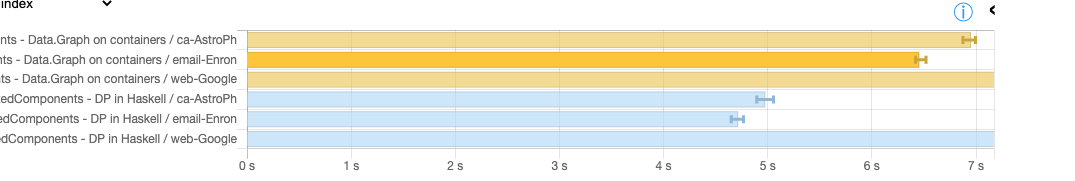
\includegraphics[width=\textwidth]{bench_1.png}
  \captionsetup{type=figure}
  \captionof{figure}{Benchmark 1 - DP in Haskell vs. Data.Graph Haskell}
  \label{fig:1}
\end{minipage}

In this first image in \autoref{fig:1} we can see that \acrshort{dp} \acrshort{hs} solution is $1.3$ faster compare with \texttt{containers} \acrshort{hs} library.

\begin{minipage}[t]{\linewidth}
  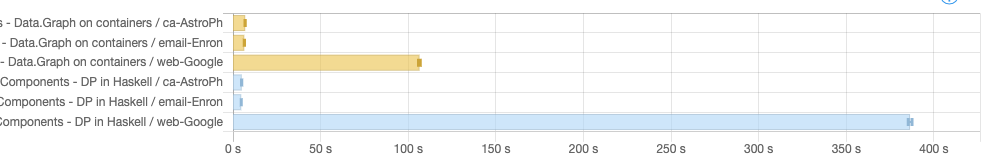
\includegraphics[width=\textwidth]{bench_2}
  \captionsetup{type=figure}
  \captionof{figure}{Benchmark 2 - DP in Haskell vs. Data.Graph Haskell}
  \label{fig:2}
\end{minipage}

On the second image in \autoref{fig:2} we are zooming in \emph{web-Google} case and, as we have stated in the \emph{E1} \autoref{table:exp:1} results, our solution is slower for all the reasons explained in \autoref{sub:sec:e1}.

Regarding mean execution times for each implementation on each case measure by \emph{criterion} benchmark we can display the following results:

\begin{table}[H]
  \centering
  \begin{tabular}{|l|l|l|l|}
   \hline
   \textbf{Network} & \textbf{\acrshort{dp}-\acrshort{hs}} & \textbf{\texttt{containers} \acrshort{hs}} & \textbf{Speed-up}\\
   \hline
   Enron Emails & 4.68s &  6.46s & 1.38\\
   \hline
   Astro Physics Coll Net & 4.98s & 6.95s  & 1.39\\
   \hline
   Google Web Graph & 386s & 106s & -3.64\\
   \hline
  \end{tabular}
 \caption{Mean Execution times}
 \label{table:6}
 \end{table}

This experiment results allows to answer Question \textbf{Q2}.
We already had a partial answer with the previous experiment \emph{E1} about \textbf{Q2} (\autoref{res:question}) where we have seen that the Topology of the Graph affect the performance and the parallelization is penalizing the solution instead of speeding up for this particular case. In doing this Benchmark Analysis the solution against a non-parallel \texttt{containers} \mintinline{haskell}{Data.Graph} confirms the hypothesis. 

\subsubsection{Diefficency Metrics}\label{sub:sub:sec:e2}
As we have commented before \acrfull{dm} Tool \emph{diefpy} \cite{diefpy} is based on the work \cite{diefpaper}. What we want to measure with this Benchmark is the ability of \acrshort{dp} Model to generate results incrementally. This is one of the strongest feature of \acrshort{dp} Paradigm since it allows process and generate results without no need of waiting for processing until last element of the input. This kind of characteristics are essential not only for big data inputs where perhaps the requirements allows processing until some point of the time having partial results, but at the same time is important to process \textit{Unbounded} streams. 

Some considerations are needed before starting to analyzed the data gathered with this tool. Firstly, the tool is plotting the results according to the traces generated by the implementation, both \acrshort{dp} in \acrshort{hs} and \emph{containers} \acrshort{hs}. By the nature of \acrshort{dp} model, we can gather or register that timestamps as long as the model is generating results. In the case of \emph{containers} \acrshort{hs} this is not possible since it calculates \acrshort{wcc} at once. This is not an issue and we still can check at what point in time all this \acrshort{wcc} in default \acrshort{hs} solutions is generated. In those cases we are going to see a straight vertical line. 

On the other hand, it is important to remark that we needed to scale the timestamps because we have taken the time in \emph{nanoseconds} because the incremental generation between one \acrshort{wcc} and the other is very small but significant to take into consideration. Therefore if we left the time scale in Integer milliseconds, microseconds or nanoseconds integer part it cannot be appreciated. In the case of the escalation we are discounting the nanosecond integer of the first generated results resulting a time scale that start close to $0$. This does not mean that first result is generate at $0$ time but we are discarding previous time because we want to focus on how the results are incrementally generated.

Having saying that, we can see the results of \acrshort{dm} which are presented in two types of plot. The first one are regular \emph{Line Graphs} in where $x$ axis shows the time escalated when the result was generated and $y$ axis is showing the component number that was generated at that time. The second type of plot is a \emph{Radar} plot in which shows how the solution is behaving on the dimensions of  \acrfull{tfft}, \acrfull{et}, \acrfull{tt}, \acrfull{comp} and \acrfull{dt} and how are the tension between them. All the details about this metrics are explained here \cite{diefpaper}.

\begin{figure}[!htb]
    \centering
    \begin{minipage}{0.33\textwidth}
     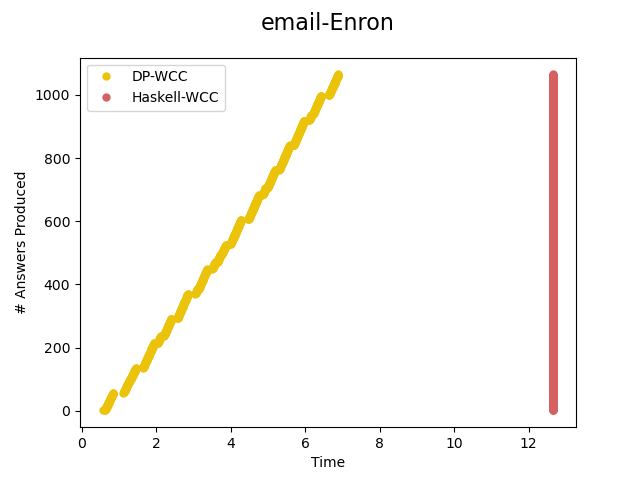
\includegraphics[width=1\linewidth, height=0.2\textheight]{email_enron}
      \caption{email-Enron \acrshort{dm}}
      \label{fig:dief:1}
    \end{minipage}%
    \begin{minipage}{0.33\textwidth}
     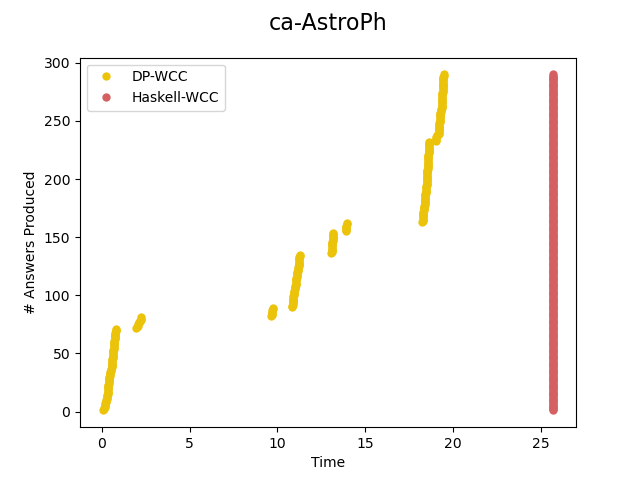
\includegraphics[width=1\linewidth, height=0.2\textheight]{ca_astroph}
      \caption{ca-AstroPh \acrshort{dm}}
      \label{fig:dief:2}
    \end{minipage}%
    \begin{minipage}{0.33\textwidth}
     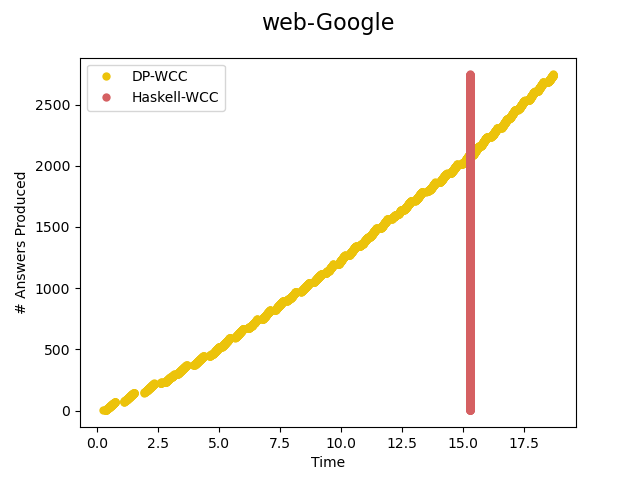
\includegraphics[width=1\linewidth, height=0.2\textheight]{web_google}
      \caption{web-Google \acrshort{dm}}
      \label{fig:dief:3}
    \end{minipage}
\end{figure}

As we can see based on the results shown in the tables above all the solutions in \acrshort{dp}-\acrshort{hs} are being generated incrementally, but there are some difference that we would like to remark. In the case of \emph{email-Enron} and \emph{ca-AstroPh} there seems to be a more incremental generation of results, in fact \emph{ca-AstroPh} is even more incremental where we can see the separation between some results and others. \emph{web-Google} Networks is a little more linear and that is because all the results are being generated with very little difference in time between them. This is due to the fact of the explained reasons in \autoref{sub:sec:e1}. Having the biggest \acrshort{wcc} at the end of \emph{web-Google} \acrshort{dp} algorithm it is retaining results until it can solve the biggest \acrshort{wcc} which takes longer. 

\begin{figure}[!htb]
    \centering
    \begin{minipage}{0.33\textwidth}
     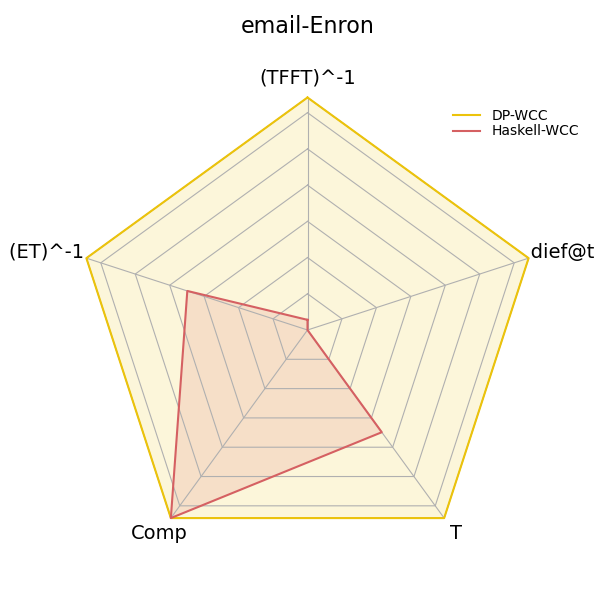
\includegraphics[width=1\linewidth, height=0.2\textheight]{email_enron_radar}
      \caption{email-Enron \acrshort{dm}}
      \label{fig:dief:rad:1}
    \end{minipage}%
    \begin{minipage}{0.33\textwidth}
     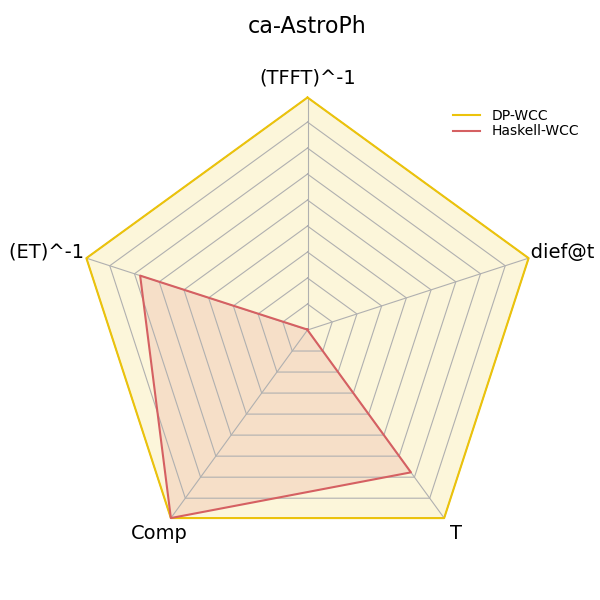
\includegraphics[width=1\linewidth, height=0.2\textheight]{ca_astroph_radar}
      \caption{ca-AstroPh \acrshort{dm}}
      \label{fig:dief:rad:2}
    \end{minipage}%
    \begin{minipage}{0.33\textwidth}
     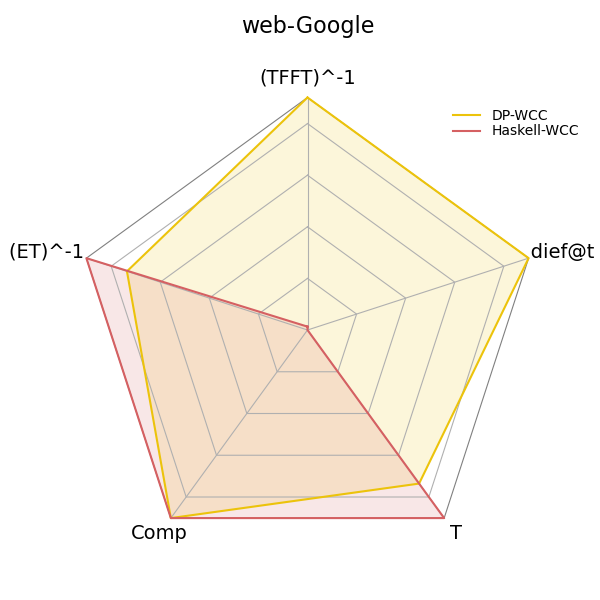
\includegraphics[width=1\linewidth, height=0.2\textheight]{web_google_radar}
      \caption{web-Google \acrshort{dm}}
      \label{fig:dief:rad:3}
    \end{minipage}
\end{figure}

As we can appreciate \emph{Radar} plots are confirming our previous analysis. We can see for example that the \acrshort{tt} of \emph{web-Google} in the case of \acrshort{dp}-\acrshort{hs} is worse than \emph{containers} in \acrshort{hs}, which is not happening for the other networks.

In conclusion we can say that regarding \textbf{Q2} (\autoref{res:question}) although we can say that \acrshort{dp} in \acrshort{hs} is faster than traditional approach, the fast execution is not always the most interest analysis that we can have, because as we have seen even when in the case of \emph{web-Google} Graph \acrshort{dp} is slower at execution, it is at least generating incremental results without need to wait for the rest of the computations.

\subsection{Experiment: E3}

For this type of analysis our experiment focus on \textit{email-Enron} Network only because profiling data generated by \textit{GHC} is big enough to conduct the analysis and on the other hand enabling profiling penalize execution time. For these reasons we have focused the profiling only on that network.

\textbf{Multithreading:} For analyzing parallelization and multithreading we have used \texttt{ThreadScope} \cite{threadscope} which allows us to see how the parallelization is taking place on \textit{GHC} at a fine grained level and how the threads are distributed throughout the different cores requested with the \mintinline{bash}{-N} execution \mintinline{bash}{ghc-option} flag.

\begin{minipage}[t]{\linewidth}
  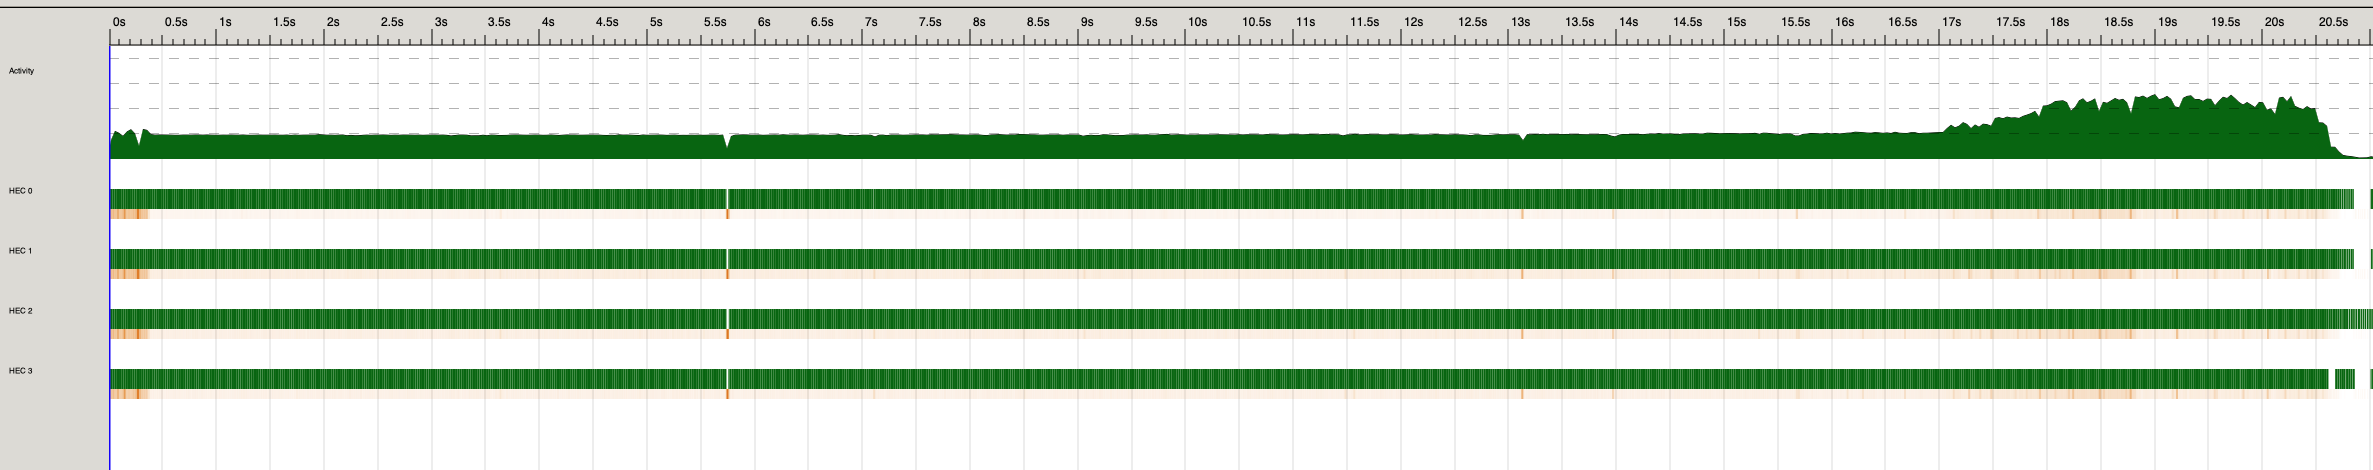
\includegraphics[width=\textwidth]{screen_1}
  \captionsetup{type=figure}
  \captionof{figure}{Threadscope Image of General Execution}
  \label{fig:3}
\end{minipage}

In this image we can see that the parallelization is being distributed evenly among the $4$ Cores that we have set for this execution.
The distribution of the load is more intensive at the end of the execution, where \mintinline{haskell}{actor2} Filter Stage \autoref{src:haskell:3} of the algorithm is taking place and different filters are reaching execution of that second Actor.

Another important aspect that we can clearly see on \autoref{fig:3} is that the amount of work is not so significant for \textit{GHC} and the threads and distribution of the work keeps between 1 or 2 cores during the execution time of the program. In this regards we can answer \emph{Research Question} \textbf{Q1 and Q3} (\autoref{res:question}), verifying that \acrshort{hs} not only supports the parallelization level required but it is evenly distributed as well across the program execution.

Finally it can also been appreciated that there is no sequential execution on any part of the program, because the $4$ cores have \texttt{CPU} activity during the whole execution time. This is due to the fact that as long the program start, and because of the nature of \acrshort{dp} model, it is spawning the \texttt{Input} Stage in a separated thread. This is a clear advantage for the model and the processing of the data since the program does not need to wait to do some sequential processing like reading a file, before start computing the rest of the stages.

\begin{minipage}[t]{\linewidth}
  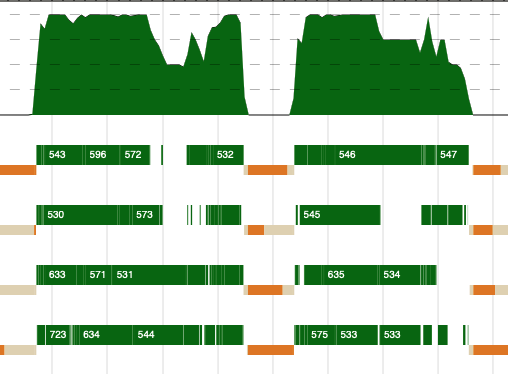
\includegraphics[width=\textwidth]{screen_2}
  \captionsetup{type=figure}
  \captionof{figure}{Threadscope Image of Zoomed Fraction}
  \label{fig:4}
\end{minipage}

In this second image on \autoref{fig:4} we are zooming in on \texttt{ThreadScope} output in a particular moment of time, approximately in the middle of the execution, in order to appreciate how many threads are being spawned and by the tool and if they are evenly distributed among cores. The numbers inside \textbf{green} bars represent the amount of \textit{Threads} that are being executed on that particular core (\textit{horizontal line}) at that execution slot. Thus, the amount of threads vary among slot execution times because as it is already known, \texttt{GHC} implements \emph{Preemptive Scheduling} \cite{lightweightghc}.

Having saying that it can be appreciated in this image \autoref{fig:4} our first assumption that the load is evenly distributed because the \textit{mean number of executing threads} are $571$.

\textbf{Memory allocation:} Another important aspect in our case is how the memory is being managed to avoid Memory Leaks or other non-desired behavior that increase memory allocation during the execution time. This is even more important in the particular implementation of \acrshort{wcc} using \acrshort{dp} model because it requires to maintain the Set of \textit{Connected Components} in memory throughout the execution of the program or at least until we can output the calculated \acrshort{wcc} if we reach to the last Filter and we know that this \acrshort{wcc} cannot be augmented anymore. 

In order to verify this, we measure memory allocation with \textit{eventlog2html} \cite{eventlog2html} which converts generated profiling memory \mintinline{bash}{eventlog} files into Graphical HTML representation. 

\begin{minipage}[t]{\linewidth}
  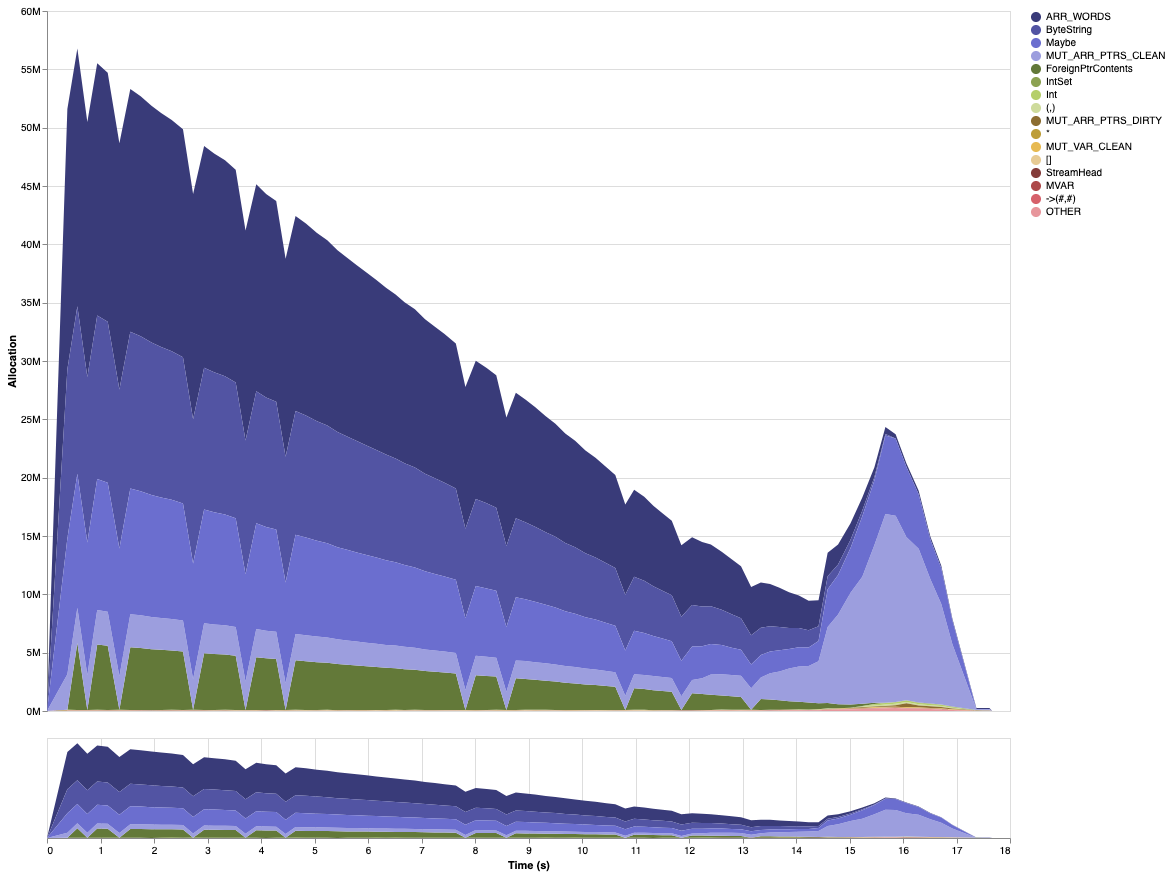
\includegraphics[width=\textwidth]{visualization}
  \captionsetup{type=figure}
  \captionof{figure}{Memory Allocation}
  \label{fig:5}
\end{minipage}

As we can see in \autoref{fig:5} our program does an optimal job on allocating memory since we are not using more than $57$ MB of memory during the whole execution of the program.

On the other hand, if we analyze how the memory is allocated during the execution of the program, it can also been appreciated that most of the memory is allocated at the beginning of the program and steadily decrease over time with a small peak at the end that does not overpass even half of the initial peak of $57$ MB. The explanation for this behavior is quite straightforward because at the beginning we are reading from the file and transforming a \mintinline{haskell}{ByteString} buffer to \mintinline{haskell}{(Int, Int)} edges. This is perfectly seen in the image in which the dark blue that are on top of the area are \mintinline{haskell}{ByteString} allocation. Light blue is allocation of \mintinline{haskell}{Maybe a} type which is the type that is returned by the \texttt{Channels} because it can contain a value or not. Remember that Data value \mintinline{haskell}{Nothing} is indicating end of the Channel as we can see here \autoref{src:haskell:3}.

Another important aspect is the \textit{green area} which represents \mintinline{haskell}{IntSet} allocation, which in the case of our program is the Datastructure that we use to gather the Set of vertices that represents a \acrshort{wcc}. This means that the amount of memory used for gathering the \acrshort{wcc} itself it minimum and it is decreasing overtime, which is another empirical indication that we are incrementally releasing results to the user. In fact it can bee seen as well that as long the green area reduces the lighter blue (\mintinline{haskell}{MUT_ARR_PTRS_CLEAN} \cite{ghcheap}) increases at the same time indicating that the computations for the output (releasing results) is taking place. 

Finally this answers Question \textbf{Q3} (\autoref{res:question}) showing that not only Memory Management was efficient not leaking or increasing memory across the running execution program.

\section{Related Work}
In \acrfull{hs} several implementations have arisen along the years to give an answer to \emph{Streaming Processing Models} \cite{pipes, conduit, streamly}. All these libraries have their own abstractions and there are able to do Data Stream Processing in a fast way with its own differences regarding execution time according to recent benchmarks \cite{benchstreamhs}. Although all these libraries seem to be suitable for implementing \acrshort{dp} model in \acrshort{hs}, all of them requires to know Pipeline Stages disposition beforehand and it is quite hard to achieve a succinct and expressive implementation of \acrshort{dp} model on such libraries. Moreover since these libraries have been conceived with a Data Pipeline Streaming model approach instead of Pipeline Stage Streaming like in \acrshort{dp} model, adapting the abstraction to these tools makes it even harder to achieve.

Another kind of \acrshort{hs} implementation is described \emph{Chapter 4} subsection \emph{Pipeline Parallelism} on this book \cite{parallelbook} in the context of \mintinline{haskell}{Par} \texttt{Monad}. On that work the author describe how to encode a Stream Pipeline parallelism with \mintinline{haskell}{Par} \texttt{Monad}. Although this could have been a proper alternative for implementing \acrshort{dp} in \acrshort{hs}, the parallelization level implemented at \mintinline{haskell}{Par} \texttt{Monad} is achieve with Sparks \citep{sparks} which is a fine grained level of parallelism inside a Thread. In \acrshort{dp} computational model we are exploring parallelization on the Pipeline Stages and not Data Parallelization, in particular the motivating example that we have explored in \autoref{sub:sec:mot:ex} is one of the algorithm in which the amount of Stages that could run in parallel is the worst case having one Stage per edge at most, but still in that escenario the amount of threads can be efficiently handled by \texttt{GHC}. Therefore there is no need of such a fine grained parallelisation level as it could be required when the data should be split in the smallest parallelizable processing units as possible. 


\section{Conclusions and Ongoing Work}
We have seen that \acrfull{dp} Paradigm implemented in \acrfull{hs} is not only suitable but also robust. We have also seen that this implementation required only few lines of code, taking advantage of already built libraries and techniques as we have describe in \autoref{sub:lib:tools}.

On the other hand, we could verify that the implementation outperforms in those cases where the topology of the graph is more sparse and where the number of vertices in the largest \acrshort{wcc} is not large (all the vertices are not in 1 big \acrshort{wcc}). This behavior is present in spite of implementing a non optimal Subgraph algorithm for the specific Problem of \acrshort{wcc}.
Moreover, we have measure using \acrshort{dt} metrics in \autoref{sub:sub:sec:e2}, the advantageous capability of \acrshort{dp} model in \acrshort{hs} implementation to deliver incremental results compare with default \texttt{containers} library implementation.
Finally we have been able to measure the principal aspects where \acrshort{dp} is Strong such as \textit{Pipeline Parallelism} and \textit{Time processing} showing that \acrshort{hs} can deal with the requirements for the problem without penalizing neither execution time nor memory allocation.
Another important aspect is that we still need to explore in deep the design and definition of the main \acrshort{dp} Framework in \acrshort{hs} taking adavantage of all the abstraction mechanisms that \acrshort{hs} provides.

In conclusion, we have gathered enough evidence to show that \acrfull{dp} Paradigm is feasible in \acrshort{hs} opening a wide range of algorithms to be explored with this Model, supported by a Pure Functional language implementation.

\bibliography{Report}

\printglossary

\appendix
\section{Automated Testing and QuickCheck}\label{apx:1}
\subsection{Automated Cases}
We have defined 6 small examples with the following particularities to be automated and be tested automatically on every run of \mintinline{bash}{stack test} or \mintinline{bash}{cabal test} depends on the selected building tool. In that sense
we are ensure the correctness of the principal algorithm on any possible modification and iteration. 

\begin{table}[H]
  \centering
  \begin{tabular}{|l|l|l|}
   \hline
   Graph case & Edges & Ordered (Edges)\\
   \hline
   1 \acrshort{wcc} & 5 & YES \\
   \hline
   1 \acrshort{wcc} & 5 & NO \\
   \hline
   2 \acrshort{wcc} & 8 & YES \\
   \hline
   1 \acrshort{wcc} & 6 & YES \\
   \hline
   3 \acrshort{wcc} & 11 & YES \\
   \hline
   3 \acrshort{wcc} & 11 & NO \\
   \hline
  \end{tabular}
 \caption{Test Cases}
 \label{table:apx:1}
 \end{table}

\begin{listing}[H]
\begin{minted}[fontsize=\small,numbers=left,frame=lines,framerule=2pt,framesep=2mm,baselinestretch=1.2,highlightlines={}]{haskell}      
it "Example 3 CC - Shuffle" $ do
  let input = "1 2\n 2 3\n 4 5\n 1 4\n 1 3\n 7 8\n 10 12\n 3 5\n 3 6\n 7 9\n 11 10\n"
  result <- liftIO $ runParallelWithExample input
  length result `shouldBe` 3
\end{minted}
\caption{Example \textit{hspec} Testing}
\label{src:haskell:6}
\end{listing}

\subsection{QuickCheck}
In this case the main challenge consist on how to write \mintinline{haskell}{Arbitrary} derivations, in order to 
allow \textit{QuickCheck} to generate a Graph $G$ and at the same time control the amount of Connected Components that we want for $G$, 
in order to verify the following property: Given a Graph $G$, $cc : G \to \mathbb{N}$ is the Function that gets the Number of Connected Components of $G$.
Then,

\begin{equation}
  \forall G, cc(G) = size(DP(G))
\end{equation}

In our QuickCheck derivation this is the following:

\begin{listing}[H]
  \begin{minted}[fontsize=\small,numbers=left,frame=lines,framerule=2pt,framesep=2mm,baselinestretch=1.2,highlightlines={}]{haskell}      
newtype Edge a = Edge (a, a)
    deriving (Show, Eq, Ord)
  
newtype Graph = Graph { _gEdges :: Set (Edge Integer) } deriving (Show)
  
instance Arbitrary (Edge Integer) where
  arbitrary = do
    v1 <- getPositive <$> arbitrary
    v2 <- (getPositive <$> arbitrary) `suchThat` (/= v1)
    return $ Edge (v1, v2)
  
arbitraryGraphs :: Gen (Graph, Int)
arbitraryGraphs = do
  amount <- choose (1, 10)
  (, amount) <$> genGraph amount
  
genGraph :: Int -> Gen Graph
genGraph = fmap Graph . genConnComp
\end{minted}
\caption{QuickCheck \acrshort{dp}}
\label{src:haskell:7}
\end{listing}

We have avoid the details of \mintinline{haskell}{genConnComp} generator function, but it basically build a Set of Edges 
in which the amount of connected components should be the amount provided by parameter, which is randomly generated by QuickCheck.
Once we have QuickCheck generator we just need to tell QuickCheck how many examples we want to test to verify our property.

\begin{listing}[H]
\begin{minted}[fontsize=\small,numbers=left,frame=lines,framerule=2pt,framesep=2mm,baselinestretch=1.2,highlightlines={}]{haskell}      
context "Property Based Testing Examples"
  $ modifyMaxSuccess (const 1000)
  $ it "Retrieves the correct number of connected components"
  $ property
  $ forAll arbitraryGraphs 
  $ \(Graph{..}, amount) -> do 
    result <- liftIO $ runParallelWithExample $ toEdgesText _gEdges
    length result `shouldBe` amount
    
\end{minted}
\caption{QuickCheck Property Verification of \acrshort{dp}}
\label{src:haskell:8}
\end{listing}


\end{document}
